
\chapter{Travail réalisé }
%\addcontentsline{toc}{chapter}{Travail réalisé}
\vspace{-1cm}
\section{Activités principales}
%\addcontentsline{toc}{section}{Activité principales}
\subsection{Projet Kaspersky Anti-Targetted Attack}
%\addcontentsline{toc}{subsection}{Projet Kaspersky Anti-Targetted Attack}

\subsubsection*{\textbf{introduction}}

\textcolor{black}{Les menaces persistantes avancées (APT) sont considérées comme des risques très dangereux pour les entreprises.}
\textcolor{black}{Il est bien entendu que les mécanismes et les techniques utilisées par les cybercriminels se développent constamment. Malgré tout cela, un trop grand nombre d'entreprises utilisent toujours d'anciennes technologies et techniques de sécurité pour contrer les menaces actuelles.}

\subsubsection*{\textbf{Pourquoi Kaspersky Anti-Targetted Attack (KATA) ?} }

\textcolor{black}{L’approche multi-niveaux de KATA aide les entreprises à mettre en œuvre une stratégie de sécurité adaptable. Grâce à l'association unique de technologies et de services consolidés par le service de veille stratégique, la solution KATA permet aux entreprises d’atténuer les risques, de détecter plus rapidement les attaques ciblées, de gérer les menaces en temps réel et d’améliorer leur protection contre de futures attaques [https://www.kaspersky.fr/enterprise-security/anti-targeted-attacks].}

\textcolor{black}{Donc les principales fonctionnalités de cette plateforme sont :}
\begin{description}
	\item [PRÉVENIR ] réduire le risque de menaces avancées et d'attaques ciblées 
	\item [DÉTECTER] identifier les activités qui pourraient signaler une attaque ciblée
	\item [RÉPONDRE] éliminer les failles de sécurité et enquêter sur les attaques 
	\item [ANTICIPER] savoir où et quand les prochaines attaques ciblés peuvent se produire
	[https://www.kaspersky.fr/enterprise-security/anti-targeted-attacks].
\end{description}

\subsubsection{Coordination du projet KATA}
%\addcontentsline{toc}{subsubsection}{Coordination du projet KATA}
\textcolor{black}{Durant toute la période de ce projet, j’ai joué le rôle d’intermédiaire entre nos équipes techniques internes et l’équipe Kaspersky pour assurer le bon déroulement, donc j’étais censé : }
\begin{itemize}
	\item Vérifier la compliance du travail réalisé par rapport au cahier de charges initiales.
	\item Assurer la fin de chaque tache dans son délai précis et donc garantir le respect des délais.
	\item Prendre en charge le reporting, les compte-rendu.
	\item Réaliser le cahier des charges.
\end{itemize}

\subsection*{\textbf{Outils utilisés :}}

\begin{description}
	\item [FreeMind] pour réaliser un plan pour les phases de projet.	\item [Microsoft Project/Excel] pour suivre le déroulement du projet et réaliser des D-GANTT
	\item [Microsoft Visio] pour réaliser les architectures réseaux et les différents diagrammes.
\end{description}
~~\\
\subsection*{Rédaction d’un cahier des charges :}

\textcolor{black}{Après avoir fait une étude réelle sur la plateforme KATA et obtenu l’expression des besoins techniques à l’aide de l’équipe réseaux et le responsable de la sécurité opérationnelle, j’ai pu rédigé un cahier des charges qui contient la présentation du produit, le périmètre, les étapes à suivre, la stratégie ainsi que l’énumération de nos contraintes techniques avérées.}
~~\\
\subsection*{Suivi du projet :}

\textcolor{black}{La première étape consistait à faire un plan pour notre projet et en tant qu’assistant chef de projet, j’étais censé :}
~~\\
\begin{enumerate}
    \item Planifier toutes les phases de projet : Suite à plusieurs réunions avec le chef de projet et l’équipe de Kaspersky, j’ai pu réaliser un plan final pour le déroulement du projet.
~~\\
\textcolor{black}{Ci-dessous une figure qui montre le plan des phases de projet réalisé avec FreeMind.}
\begin{figure}[H]
	\begin{center}
		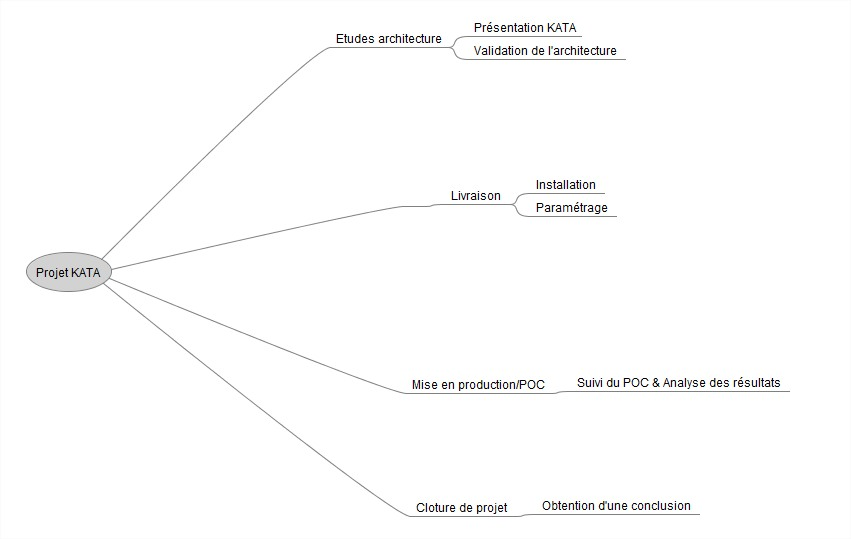
\includegraphics[width=1\linewidth]{Projet_KATA/freeMind}
\end{center}
	\caption{phases du projet}
	\label{fig:4}	
\end{figure}
		 
\item Suivre le déroulement du projet et réaliser le gestion des risques,des actions, des délais ansi que les décisions prises durant le projet. 

\textcolor{black}{Ci-dessous une capture sur le document.}
\begin{figure}[H]
	\begin{center}
		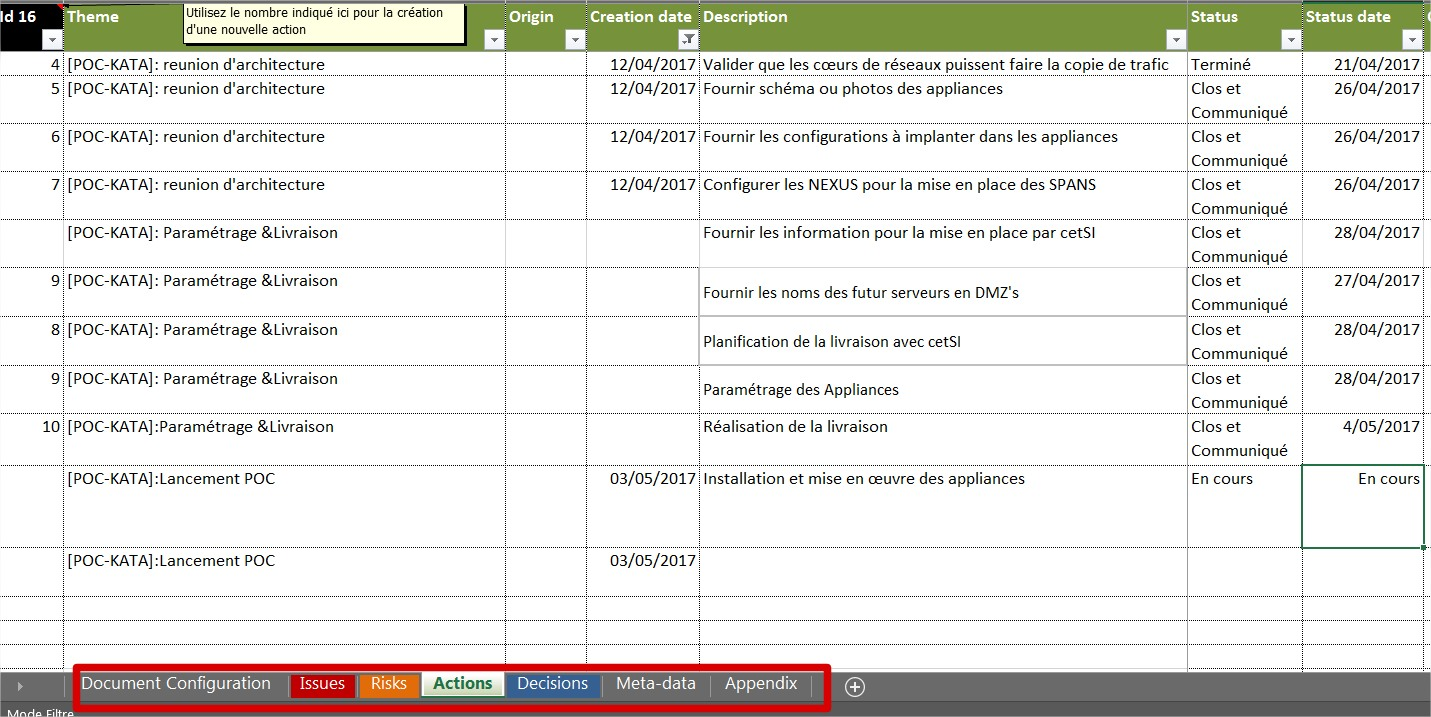
\includegraphics[width=1\linewidth]{Projet_KATA/suiviExcel}
\end{center}
	\caption{Capture sur l'un des fichiers de suivi du projet}
	\label{fig:5}	
\end{figure}
		 
\item Réaliser un diagramme de Gant en utilisant Microsoft Project pour assurer la fin de chaque tache dans son délai précis et donc garantir le respect des délais.
~~\\
\textcolor{black}{Ci-dessous une capture sur le document.}
\begin{figure}[H]
	\begin{center}
		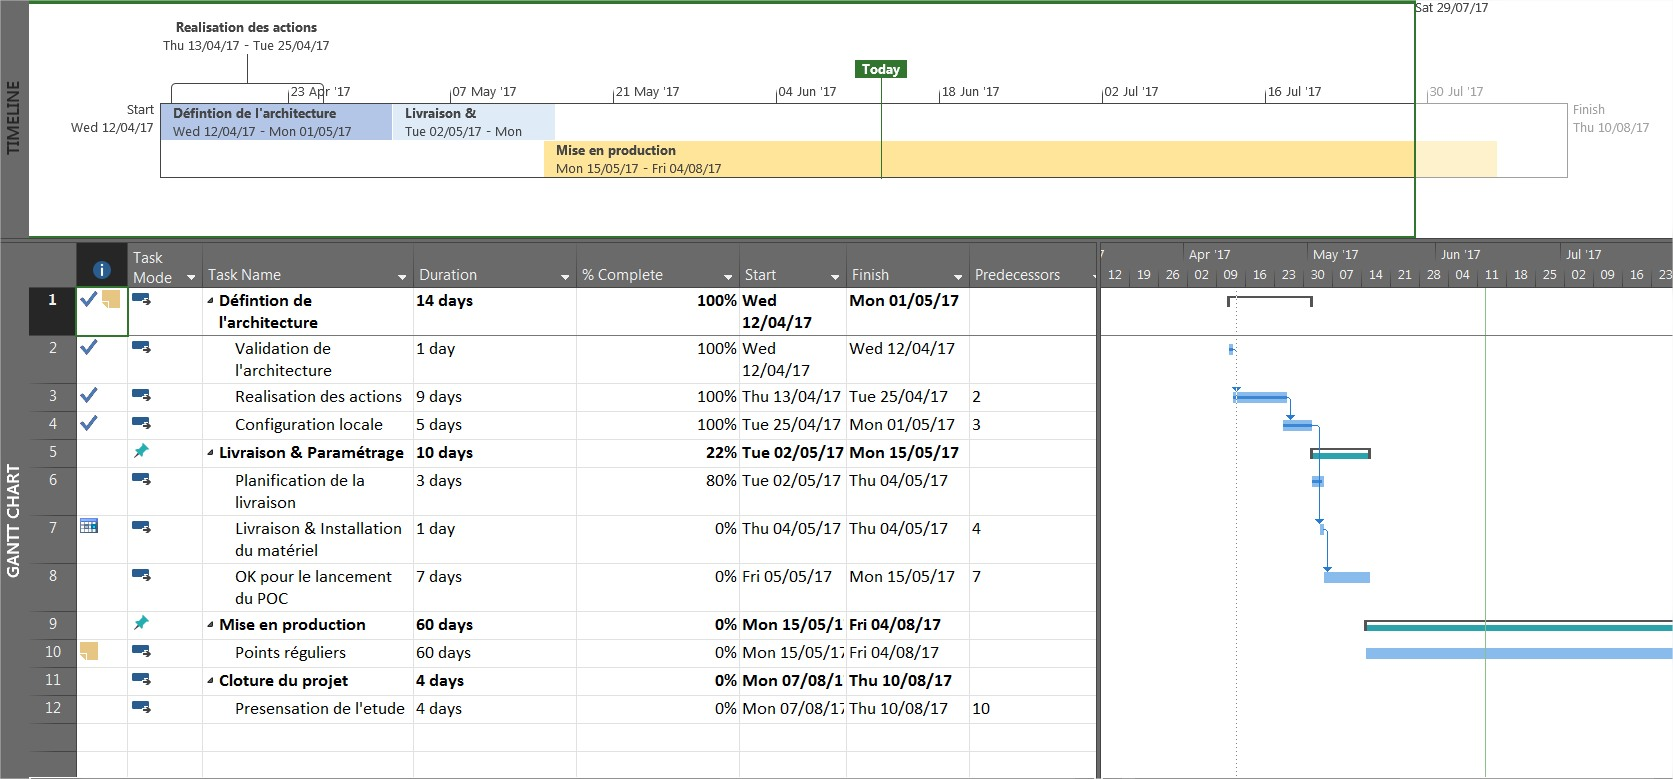
\includegraphics[width=1\linewidth]{Projet_KATA/MSproject}
\end{center}
	\caption{Capture sur le document "Project" de suivi du projet }
	\label{fig:5}	
\end{figure}		 
		 
\end{enumerate}
\vspace{0.5cm}
\subsubsection{Validation de l’architecture}
\vspace{0.5cm}
%\addcontentsline{toc}{subsubsection}{Validation de l’architecture}
\textcolor{black}{Plusieurs réunions ont été organisées avec l’équipe réseaux, sécurité et l’équipe Kaspersky afin d’étudier et valider l’architecture avant la mise en place des serveurs dans leurs locaux.}
\textcolor{black}{Suite à ces réunions, j’ai pu faire un document qui contient les décisions, les actions ainsi que les risques et qui a été ensuite validé par les responsables.}

\textcolor{blck}{ Enfin, et à l’aide de l’équipe réseaux, j’ai réalisé une architecture qui répond aux besoins mentionnés dans le cahier des charges et qui se résume dans la description suivante :}
\vspace{0.5cm}

\textcolor{black}{Nous avions besoin des rôles suivants :}

\begin{description}
	\item [Central – Node] le central node permet de synthétiser les traitements des sensors, de récupérer les informations du Kaspersky Security Network, de transmettre les éléments à tester dans la sandbox et de transmettre les alertes.
	\item [Sensor] Un sensor permet la récupération des flux, leur traitement et de transmettre l’information au Central Node.
	\item [Sandox] elle permet de tester les fichiers, url, scripT , dans un environnement connecté sur Internet et protégé du réseau de production.
	
\end{description}
	
~~\\
~~\\
\textcolor{black}{Kaspersky met à disposition 3 appliances physiques. Dans une configuration optimale, avec l’application en production, il faudrait avoir au minimum une appliance à Courbevoie et une autre à Nanterre, ceci afin de capturer l’ensemble des flux réseaux.}

\begin{figure}[H]
	\begin{center}
		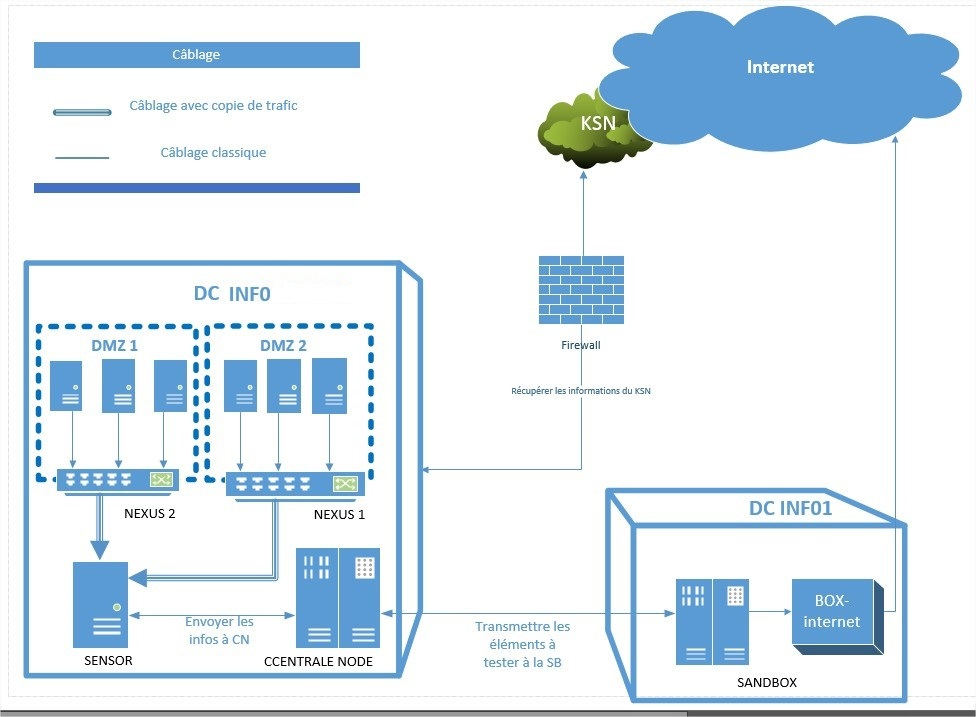
\includegraphics[width=0.9\linewidth]{Projet_KATA/archi_kata}
\end{center}
	\caption{Capture sur l’architecture réalisé avec « Microsoft Visio »}
	\label{fig:6}	
\end{figure}		 
		 
\subsubsection{Configuration des serveurs }
%\addcontentsline{toc}{subsubsection}{Configuration des serveurs }

\textcolor{black}{Après avoir assuré la livraison et la mise en production des 3 appliances (Sensor, SandBox, Central Node), j’étais censé les configurer à l’aide de PUTTY qui est un émulateur de terminal doublé d'un client pour les protocoles SSH, Telnet, rlogin, et TCP brut [Https://fr.wikipedia.org/wiki/PuTTY].}

\textcolor{black}{Ci-dessous 2 captures qui montrent la première phase de configuration.}

\begin{figure}[H]
	\begin{center}
		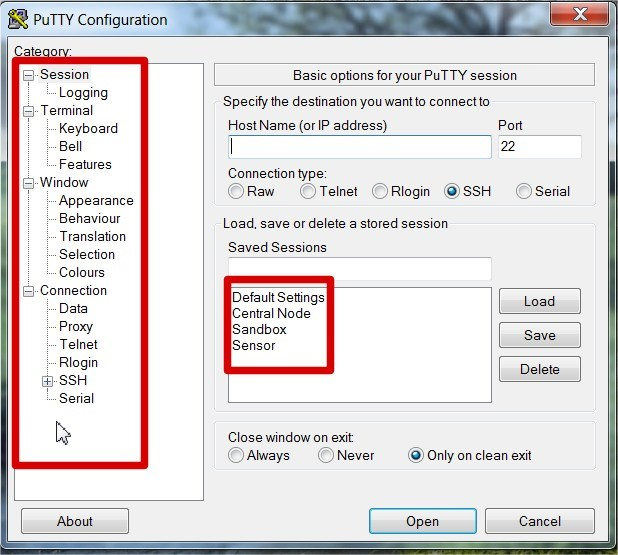
\includegraphics[width=0.8\linewidth]{Projet_KATA/iPutty}
\end{center}
	\caption{Interface de l'emulateur PUTTY}
	\label{fig:7}	
\end{figure}
\textcolor{black}{172.16.254.1: Adresse IP Centrale Node.}
\begin{figure}[H]
	\begin{center}
		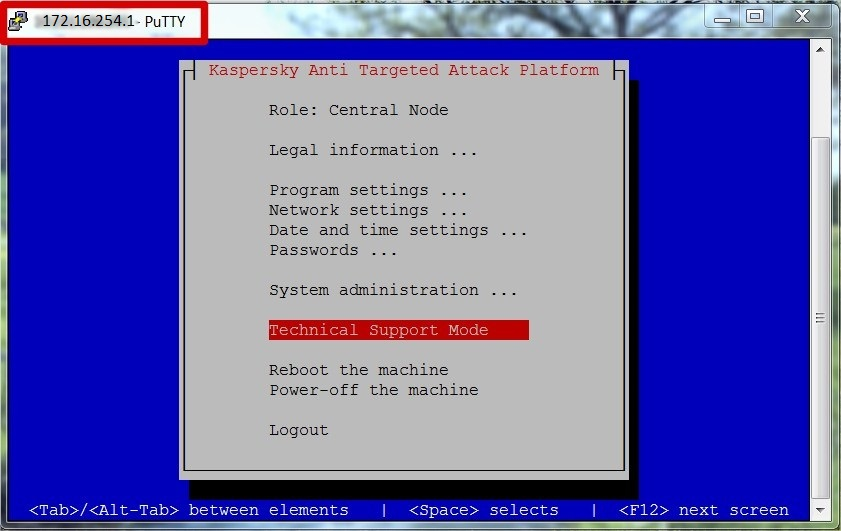
\includegraphics[width=0.8\linewidth]{Projet_KATA/Putty}
\end{center}
	\caption{Capture sur la premiére phase de la configuration de Centrale-Node}
	\label{fig:8}	
\end{figure}		 
		 
\subsubsection{Suivi du POC KATA. }
%\addcontentsline{toc}{subsubsection}{Suivi du POC KATA. }
\textcolor{black}{Après la mise en production et la configuration des serveurs, j’ai eu l’accès à la console Kaspersky Anti Targeted Attack et ce qui m’a permis de suivre les évènements et analyser les données. }
\textcolor{black}{Au début, on a reçu un grand nombre d'évènements (environs 2 millions), mais 99,65\% de ces évènements étaient des fausses alertes (demande de résolution DNS) et donc j’étais censé faire une Black-Liste des domaines concernés et la fournir à l’équipe réseaux pour qu’ils mettent à jour la stratégie globale de Firewall.}

\textcolor{black}{Pour la liste des autres domaines suspects signalés par KATA, je vérifiais toujours les nouveaux domaines indiqués et je voyais les adresses IP des machines concernées en cherchant aussi leurs localisations via IPAM (IP Adress Management), afin de faire un rapport quotidien et le fournir au responsable de sécurité. }

\textcolor{black}{Ci-dessous une capture sur la console KATA.}

\begin{figure}[H]
	\begin{center}
		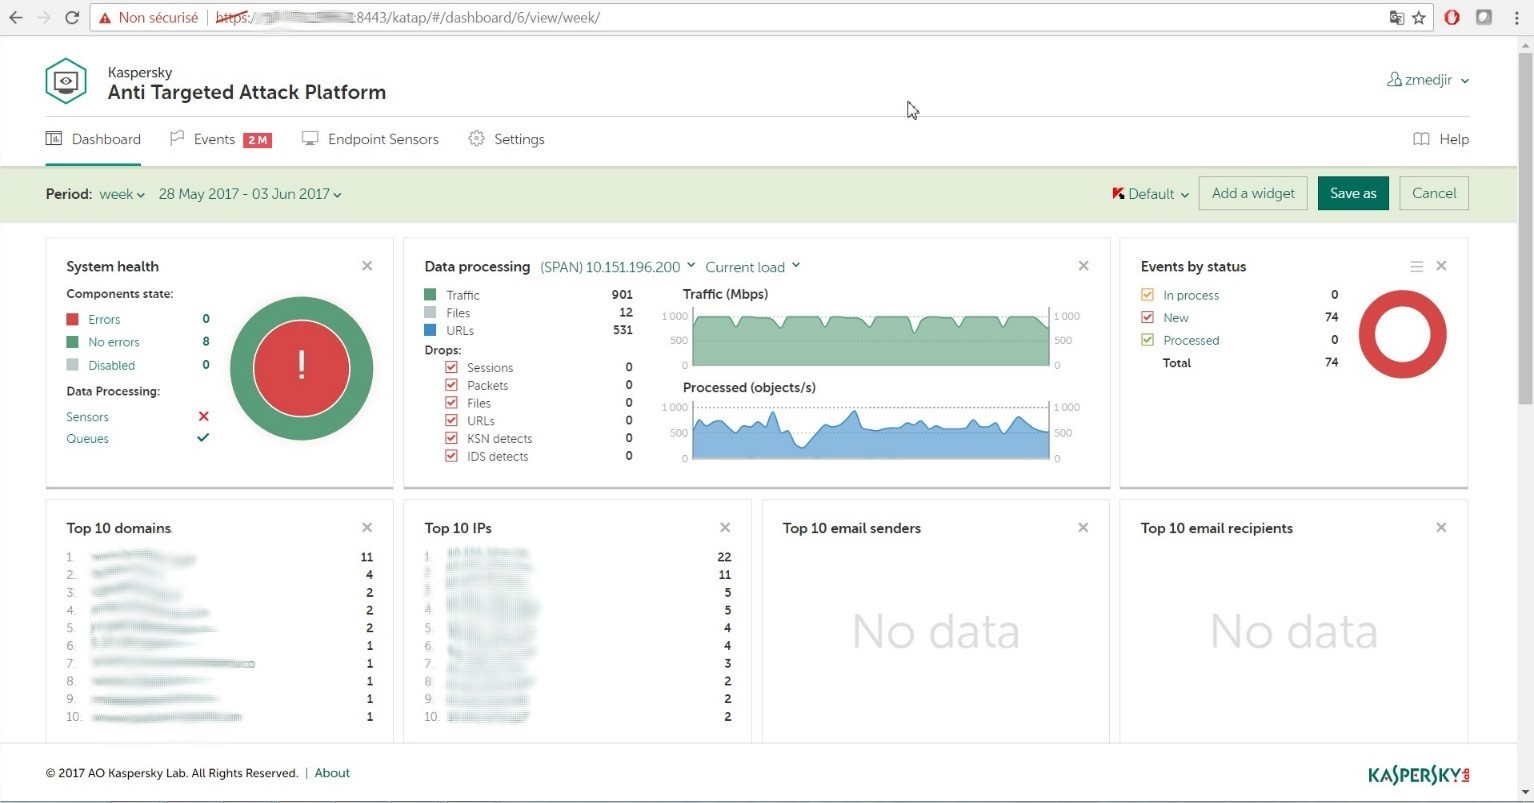
\includegraphics[width=1\linewidth]{Projet_KATA/console_kata}
\end{center}
	\caption{Console Kaspersky Anti Targeted Attack}
	\label{fig:9}	
\end{figure}		 
		 

\textcolor{black}{Avec l’option d’exportation des évènements, j’ai pu avoir un fichier excel qui contient toutes les données et donc ça m'a permis ensuite de les analyser et de réaliser des rapports.}

\begin{figure}[H]
	\begin{center}
		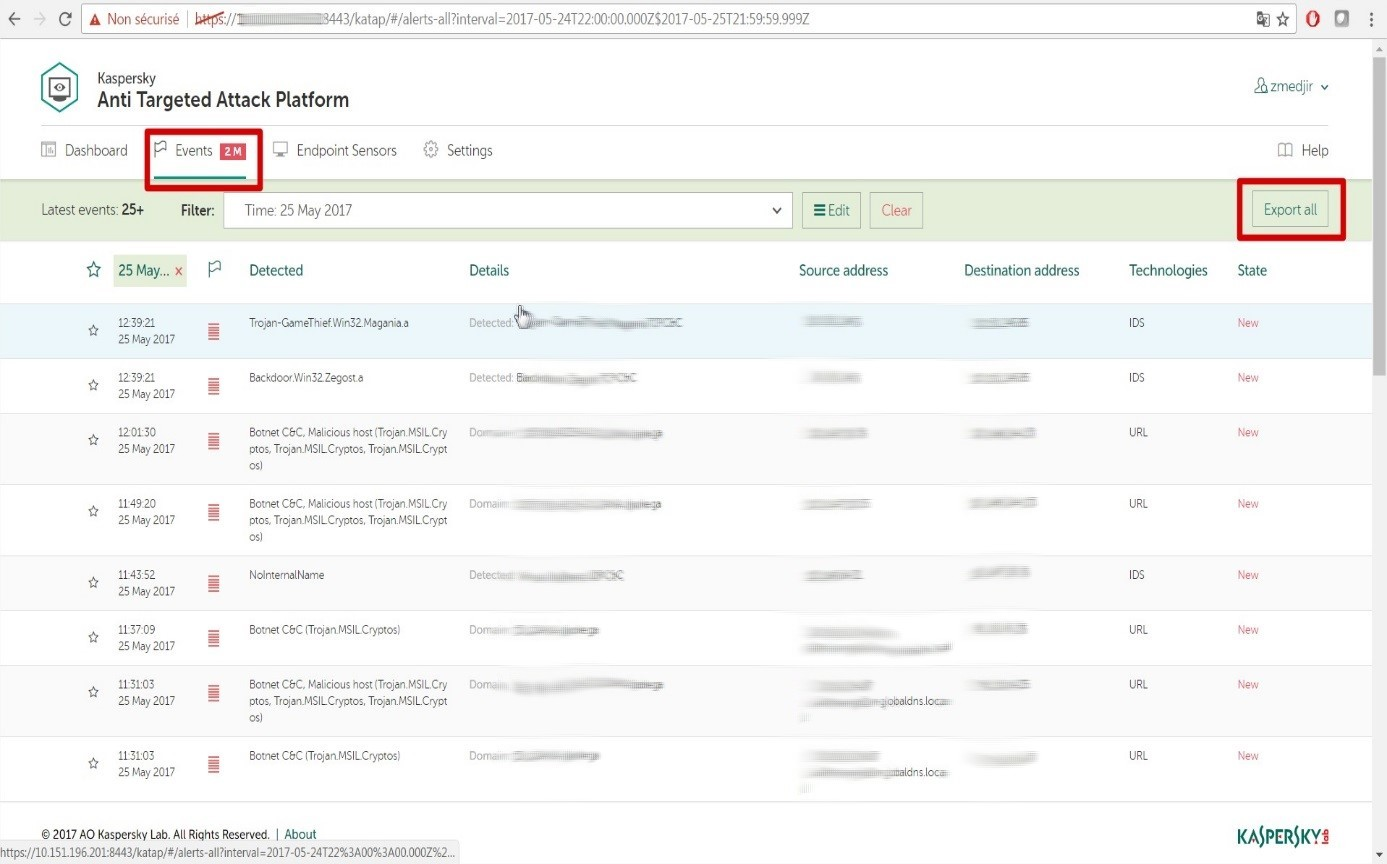
\includegraphics[width=1\linewidth]{Projet_KATA/export_kata}
\end{center}
	\caption{Capture sur la possibilité d'exportation des données}
	\label{fig:10}	
\end{figure}		 
		 
\subsubsection{Rédaction des rapports d’incidents}
%\addcontentsline{toc}{subsubsection}{Rédaction des rapports d’incidents}

\textcolor{black}{Je faisais des points tous les 3 jours avec l’équipe réseaux ainsi que l’équipe sécurité et je leurs montrais un compte rendu sur ce qu’on reçoit comme éventements pour qu’ils entament les démarches nécessaires de leurs parts afin de contrôler la situation.}	

\textcolor{black}{Ci-dessous une capture qui montre l’analyse des données d’une période de 3 jours via les tableaux croisés sous excel.}

\begin{figure}[H]
	\begin{center}
		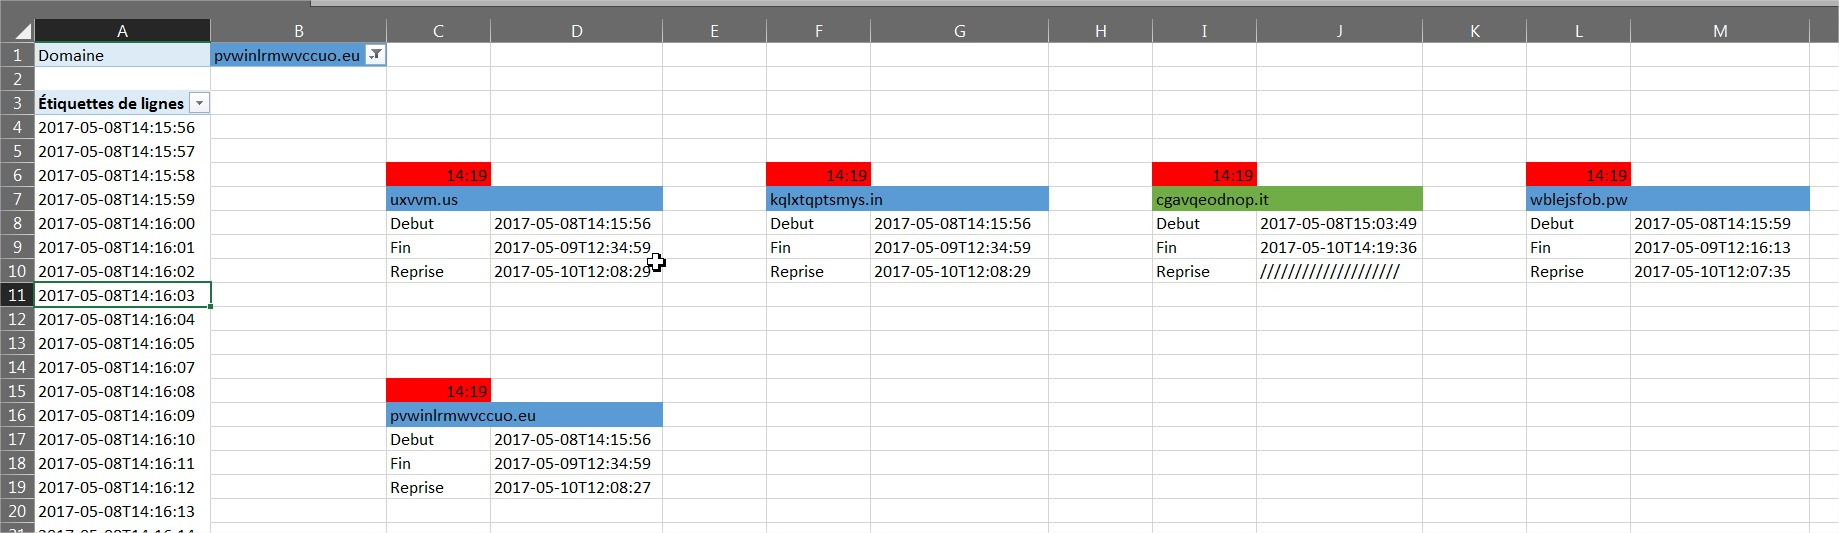
\includegraphics[width=1\linewidth]{Projet_KATA/rapport_excel}
\end{center}
	\caption{Tableaux croisés sous excel}
	\label{fig:11}	
\end{figure}	
		 		 
		 		 
\begin{figure}[H]
	\begin{center}
		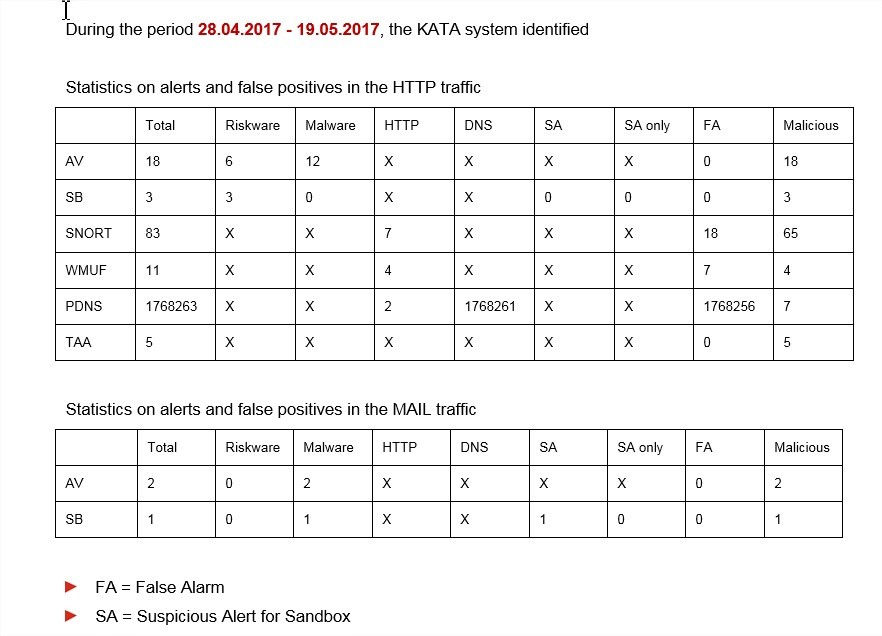
\includegraphics[width=1\linewidth]{Projet_KATA/rapport_ksy}
\end{center}
	\caption{Un exemple sur un rapport de 3 semaines.}
	\label{fig:12}	
\end{figure}	
~~\\

\subsection{Projet migration OFFICE 365}
%\addcontentsline{toc}{subsection}{Migration OFFICE 365}
\subsubsection*{introduction}

\textcolor{black}{Le projet consiste à effectuer une migration de 32 000 boites aux lettres Exchange vers Office 365 et aussi une migration Skype for Business sur un périmètre de 5 continents (105 pays).}

\subsection*{Travail demandé	}


\textcolor{black}{Faire la gestion des lotissements pour définir les listes des personnes qui ont migrées ainsi que les personnes qui devront migrer dans chaque lot de migration.
Les contraintes pourront être métier or organisationnelles telles que les membres d’une même équipe, les assistantes et leur patron, les boites aux lettres partagées, les personnes VIP, VOP etc.}

\textcolor{black}{Donc l’objectif est de :}

\begin{itemize}
	\item Consolider les données et concevoir une base de référence dynamique à partir des fichiers Excel.
	\item Analyser les données
	\item Réaliser des tableaux de bord pour l'évaluation de l'organisation des opérations effectuées.
\end{itemize}
~~\\ 
 	
\subsection*{Solution Proposée}

\textcolor{black}{Suite à l’étude des besoins que j’ai réalisé, et vu que je maitrise bien les outils décisionnels, je leurs ai proposé de faire ce travail avec POWER BI qui est un outil d’analyse et de restitution de l’information décisionnelle qui permet de :}



\begin{itemize}
	\item Faire l’extraction et la transformation des données depuis différentes sources de données.
	\item Consolider et unifier toutes les données de notre organisation, qu’elles se trouvent dans le cloud ou qu’elles soient stockées localement
	\item Réaliser des modèles de données
	\item Concevoir des rapports interactifs.
	\item Concevoir des tableaux de bords personnalisés.
\end{itemize}


\textcolor{black}{Le point fort de cet outil, c’est de pouvoir publier les rapports et les tableaux de bords créés en les partageant avec les autres collaborateurs du projet.}

\textcolor{black}{Un autre point aussi, c’est la mise à jour automatique après chaque modification faite sur l’un des fichiers sources locaux ou ceux qui se trouvent sur le cloud.}

\begin{figure}[H]
	\begin{center}
		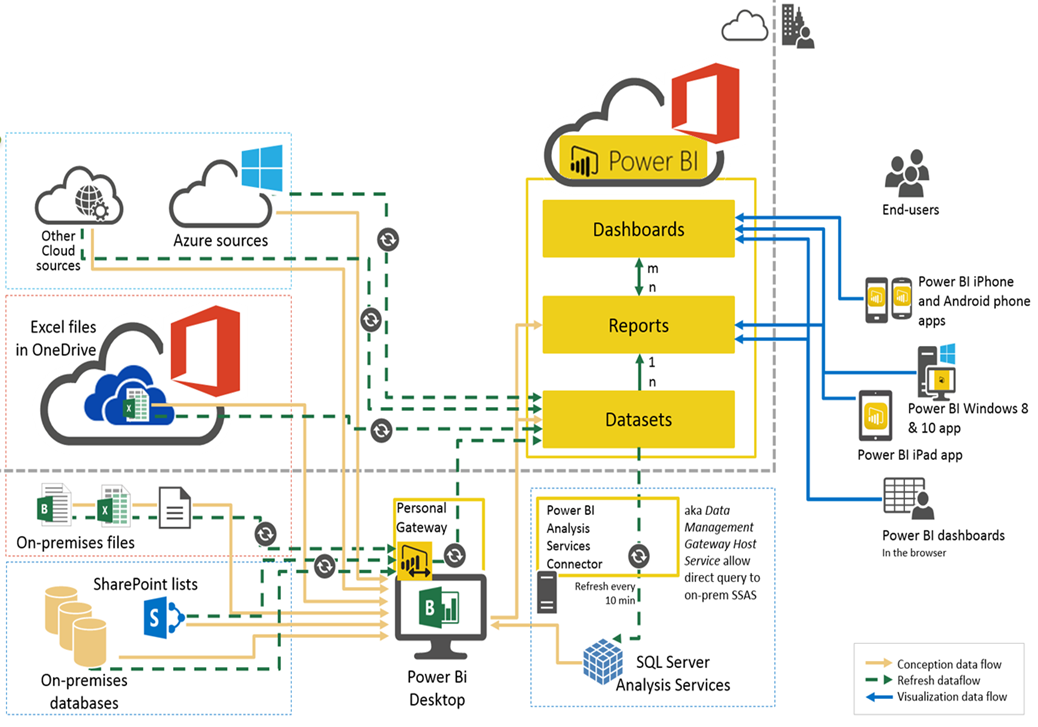
\includegraphics[width=1\linewidth]{Projet_O365/archi_BI}
\end{center}
	\caption{Architecture globale de POWER BI}
	\label{fig:12}	
\end{figure}	

\subsection*{Réalisation du système décisionnel}

\textcolor{black}{L’implémentation de notre solution s’effectue selon les quatre étapes suivantes :
\begin{itemize}
	\item   Construction de l’entrepôt de données ;
	\item	Mise en place des processus ETL ;
	\item	Réalisation des cubes dimensionnels ;
	\item	Création des rapports.
\end{itemize}
}
		 	
\subsubsection{Le processus ETL (Extraction, Transformation et Chargement)}
%\addcontentsline{toc}{subsubsection}{Le processus ETL (Extraction, Transformation et Chargement)}

\textcolor{black}{
Afin d’exploiter les données pour la prise de décision, il faut les rassembler dans une même zone, et comme les données de l’entreprise se trouvent dans plusieurs endroits alors on utilise un outil ETL pour les rassembler.}

\textcolor{black}{
Selon (Poletto, 2012), un ETL extrait, nettoie, et importe les données à partir de  différentes sources et les charge dans un entrepôt de données.}
\textcolor{black}{
A partir de cette définition, nous distinguons les trois étapes d’un processus ETL :}

\subsubsection*{Extraction}
%\addcontentsline{toc}{subsubsubsection}{Extraction}

\textcolor{black}{
 « L’extraction est la première étape du processus d'apport de données à l'entrepôt de données. Extraire, cela veut dire lire et interpréter les données sources et les copier dans la zone de préparation en vue de manipulations ultérieures » (Kimball et Ross, 2013).}

\textcolor{black}{
 Cette étape consiste à identifier les données pertinentes pour l’aide à la décision à partir des différentes sources et puis les extraire et les charger dans la zone de préparation de données en vue de les transformer et les rendre exploitables par les décideurs.}

\textcolor{black}{
 L’extraction, lors de la première fois, se fait sur l’intégralité des données de l’entreprise. Puis, des extractions périodiques seront planifiées afin de collecter les nouvelles données ou celles ayant changé.}

\subsubsection*{Transformation}
%\addcontentsline{toc}{subsubsubsection}{Transformation}

\textcolor{black}{
La transformation est la deuxième étape du processus ETL.  Avant de charger les données dans l’entrepôt de données, il est nécessaire d’appliquer un ensemble d’opérations sur les données extraites afin de les épurer et les rendre exploitable.}
\textcolor{black}{
Les opérations en question peuvent être :}

\begin{itemize}
	\item Nettoyage de données par l’application des filtres, la suppression des doublons, le traitement des valeurs nulles et la correction des erreurs.
	\item	Affectation des clés de substitution aux dimensions.
	\item	Contrôle d’intégrité en assurant la correspondance entre les clés primaires des dimensions et les clés étrangères des tables de faits.
	\item	Agrégation de données en calculant les moyennes, les sommes, le maximum, le minimum et les comptages selon le niveau de granularité souhaité.
	
\end{itemize}

\subsubsection*{Chargement}
%\addcontentsline{toc}{subsubsubsection}{Chargement}

\textcolor{black}{
Le chargement de données est la dernière étape du processus ETL. Elle consiste à transférer les données transformées à l’entrepôt de données. }
\textcolor{black}{
Nous distinguons deux types de chargement :}

\begin{itemize}
	\item \textbf{Chargement initial :} Ce type est appliqué une seule fois dans le cycle de vie du système décisionnel. Il consiste à charger toutes les données opérationnelles de l’entreprise dans l’entrepôt de données. Ce type peut être refait dans les cas particuliers comme la perte de toutes les données de l’entrepôt.

    \item \textbf{Chargement incrémental :} Ce type de chargement se fait périodiquement et automatiquement en vue de charger les nouvelles données ou les données qui ont subi des changements.
\end{itemize}

~~\\

\subsubsection{Consolidation des données en un base de référence }
%\addcontentsline{toc}{subsubsection}{Consolidation des données en un base de référence}
\textcolor{black}{Afin d’exploiter les données pour la prise de décision, il faut les rassembler dans une même zone, et comme les données de l’entreprise se trouvent dans plusieurs endroits alors on utilise un outil ETL pour les rassembler.}
\textcolor{black}{Suite à plusieurs réunions organisées avec l’équipe AVANADE (cellule chargé de faire la migration O365), j’ai eu toutes informations nécessaires qui me permettent de concevoir une base de référence.}
\textcolor{black}{Les données sont stockées dans des fichiers Excel, chaque fichier contient plusieurs feuilles, l’adresse mail est la colonne clé dans notre modèle de donnée et donc nous nous focalisons sur la connexion POWER BI – EXCEL.}


\begin{figure}[H]
	\begin{center}
		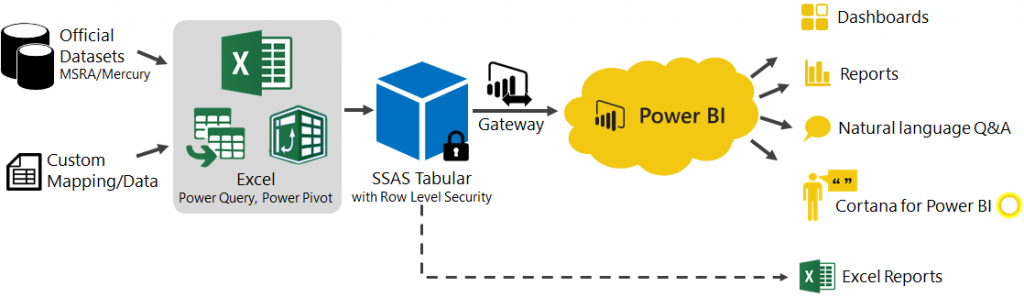
\includegraphics[width=0.8\linewidth]{Projet_O365/archi_bi_excel}
\end{center}
	\caption{Architecture du modèzle POWER BI - EXCEL}
	\label{fig:13}	
\end{figure}

\subsection*{Mise en place des processus ETL}

\textcolor{black}{La première étape consiste à faire l’extraction des données depuis les fichiers Excel concernés tels que chaque feuille représente une table dans le modèle de données avec la possibilité de combiner des données venant de plusieurs fichiers différents et de les mettre en forme en fonction des besoins, puis de les consolider dans une seule table utile.}
\begin{figure}[H]
	\begin{center}
		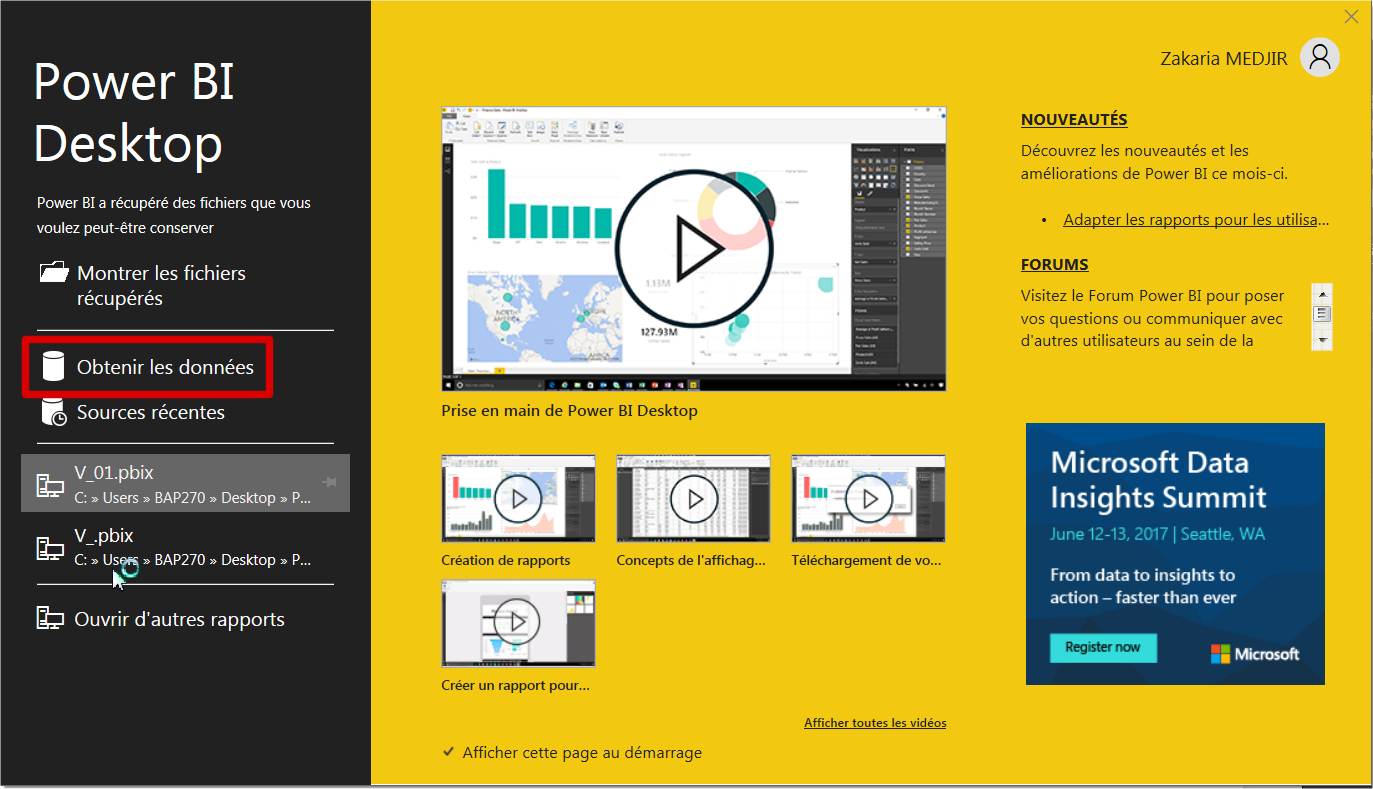
\includegraphics[width=0.70\linewidth]{Projet_O365/extraction}
\end{center}
	\caption{Exemple sur l’extraction des données depuis un fichier Excel sous POWER BI.}
	\label{fig:14}	
\end{figure}
~~\\
\textcolor{black}{Après l’extraction nous passons à la phase de transformation avant  le chargement des données.}

\begin{figure}[H]
	\begin{center}
		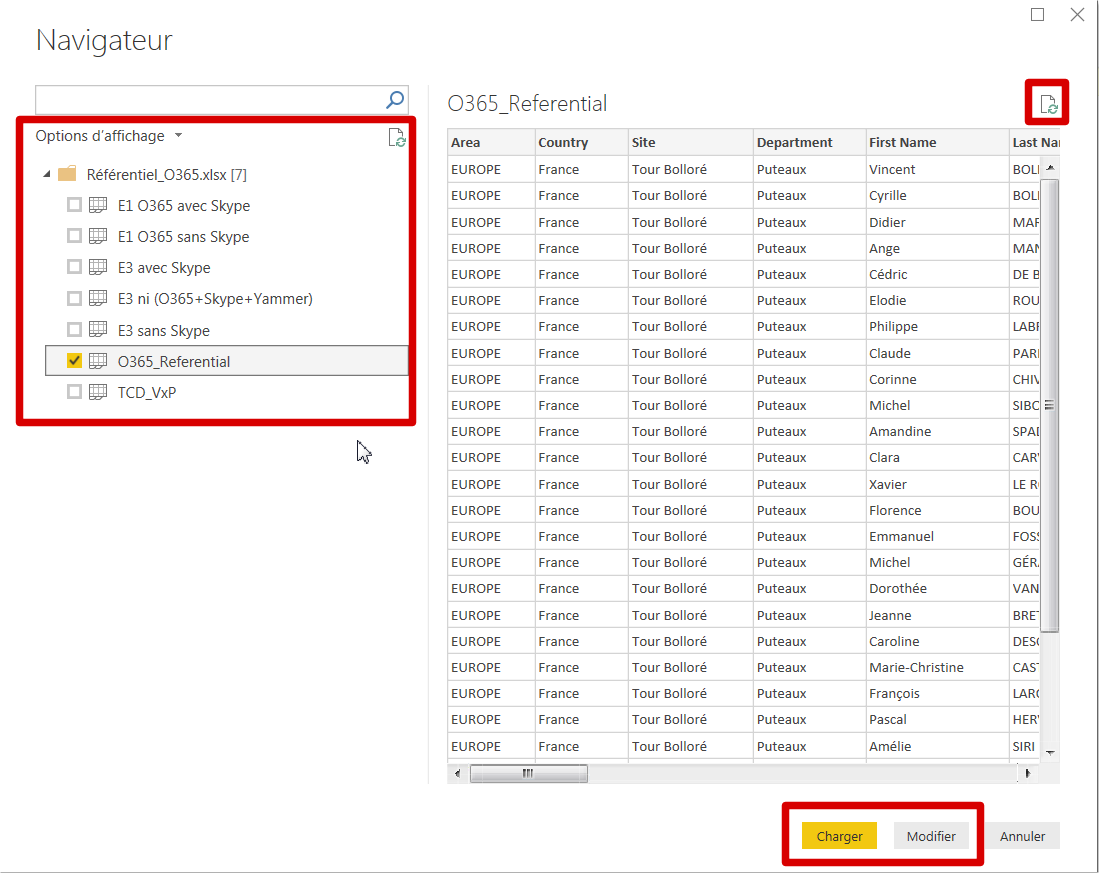
\includegraphics[width=0.8\linewidth]{Projet_O365/modification}
\end{center}
	\caption{Exemple sur la transformation sous POWER BI}
	\label{fig:15}	
\end{figure}

\begin{figure}[H]
	\begin{center}
		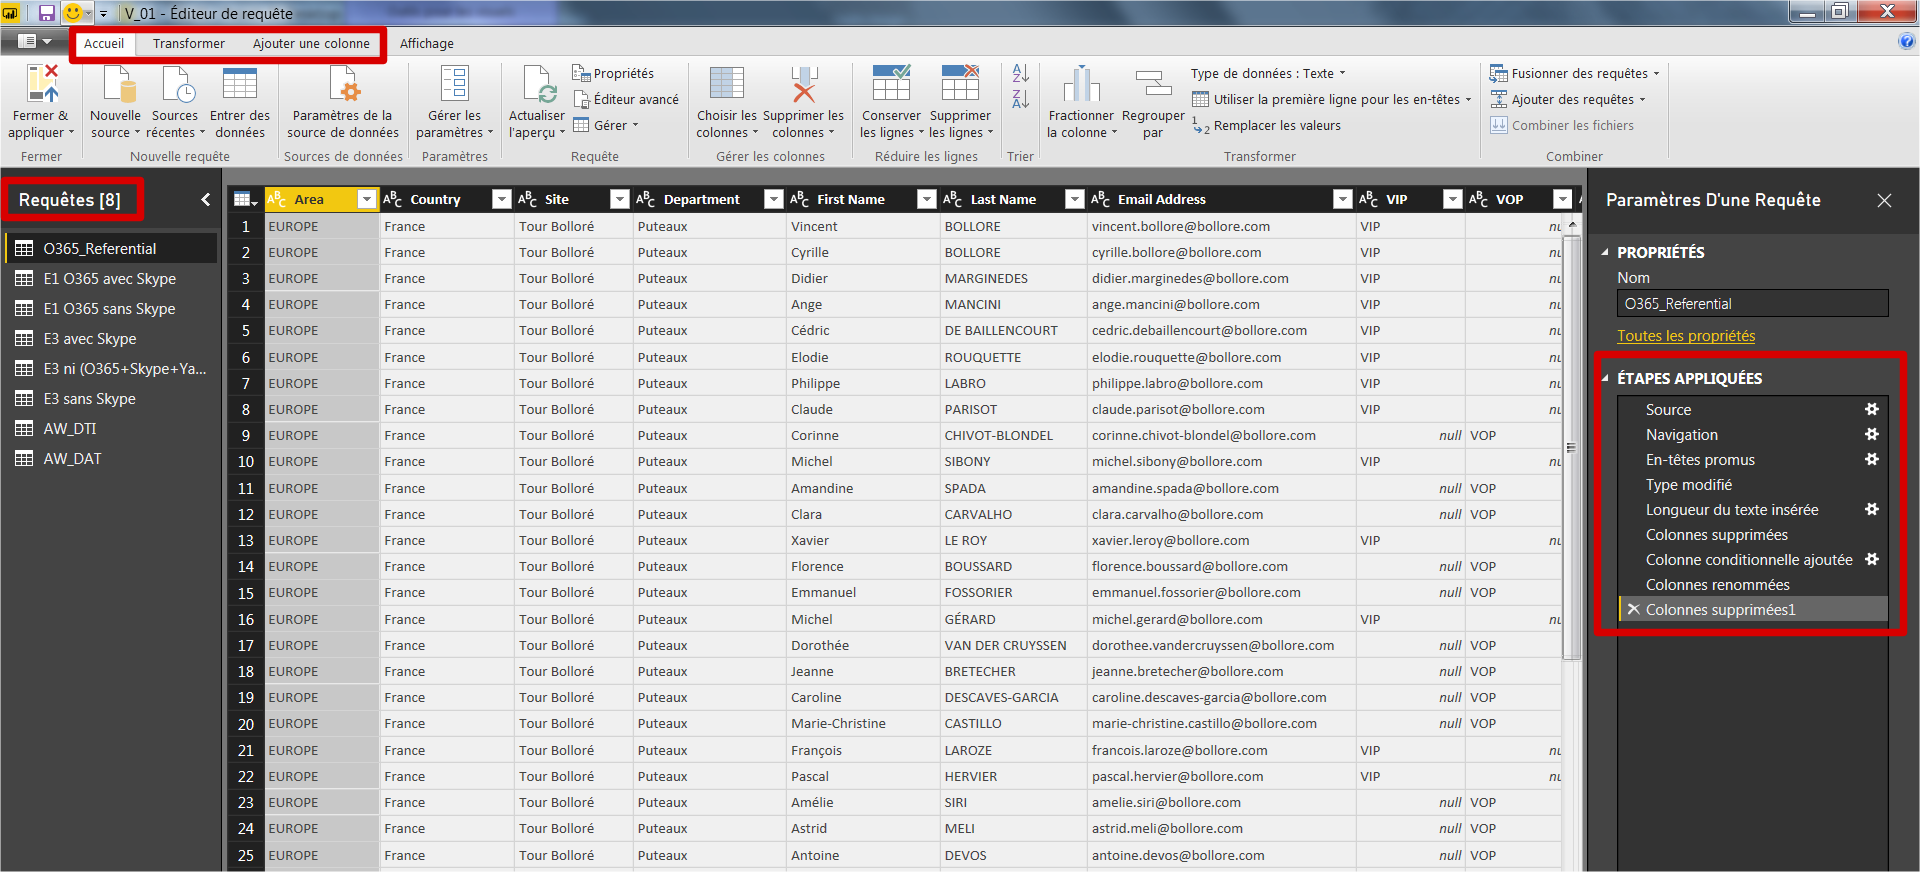
\includegraphics[width=0.8\linewidth]{Projet_O365/transformaion}
\end{center}
	\caption{Exemple  sur la transformation sous POWER BI}
	\label{fig:16}	
\end{figure}



\subsubsection{Les entrepôts et magasins de données}

\textcolor{black}{Grâce au processus ETL, les données sont stockées et organisées dans un entrepôt de données. Le
concept d’entrepôt de données a été introduit car les bases de données transactionnelles ne répondent
pas aux besoins d’analyse}

\textcolor{black}{La prochaine phase consite à gérer les relations entre toutes les tables qui ont été déjà créés et donc concevoir un model conceptuel de donnée formé en fonction des besoins.}

\textcolor{black}{Voici un exemple qui montre un modèle de donnée obtenu après la gestion des relations.}

\begin{figure}[H]
	\begin{center}
		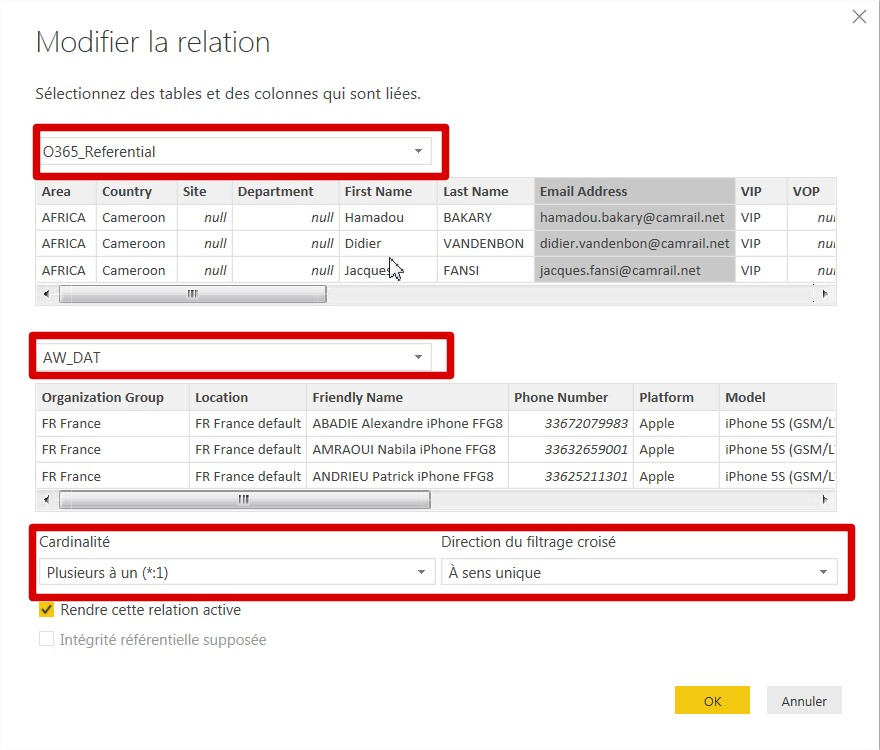
\includegraphics[width=0.7\linewidth]{Projet_O365/jointure}
\end{center}
	\caption{Exemple sur une jointure entre 2 tables.}
	\label{fig:17}	
\end{figure}

\begin{figure}[H]
	\begin{center}
		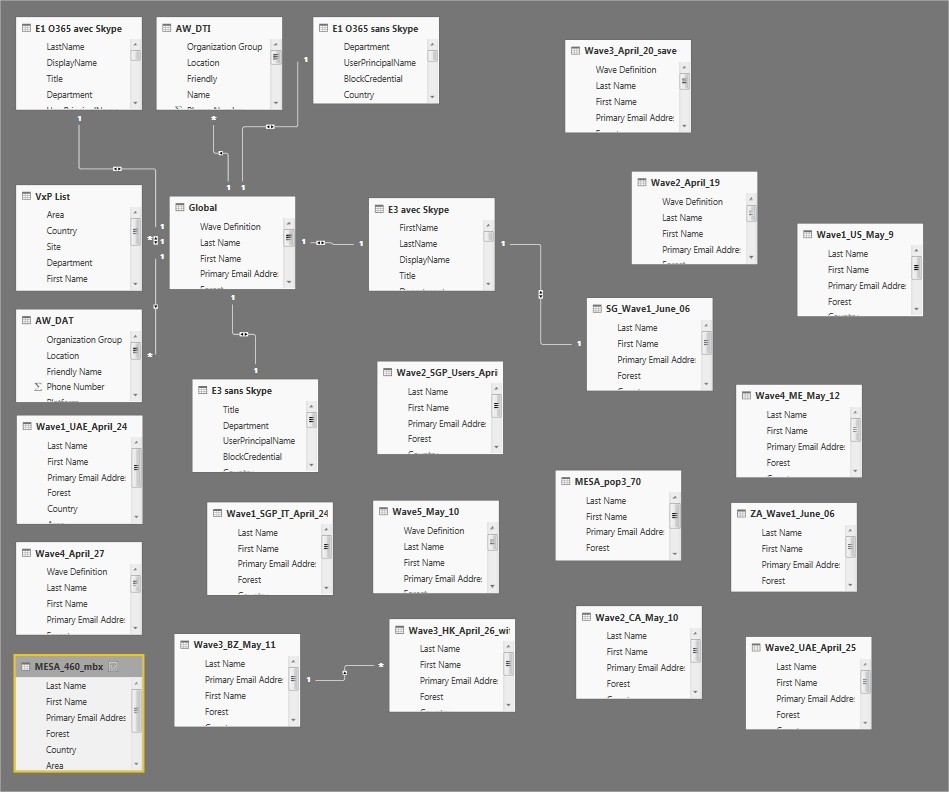
\includegraphics[width=0.8\linewidth]{Projet_O365/modele}
\end{center}
	\caption{Exemple sur un modéle des tables obtenu}
	\label{fig:18}	
\end{figure}


\subsubsection{Reporting \& Tableaux de bord }
%\addcontentsline{toc}{subsubsection}{Reporting \& Tableaux de bord }

\textcolor{black}{Le dernier niveau est l’interface qui permet aux utilisateurs d’interagir avec leur système décisionnel.C’est l’élément qui les intéressent le plus parce qu’il leur permet d’exploiter et d’analyser les données
stockées.}

\subsubsection*{Le reporting }

\textcolor{black}{Le reporting est l’ensemble des comptes rendus permettant à une entreprise de suivre son activité.
Cela permet à l’entreprise de s’évaluer grâce à la création périodique de rapports et de bilans analytiques
sur son activité. Ces rapports sont souvent destinés au manager ou au corps exécutif (Poletto, 2012).}

\textcolor{black}{ Ces comptes rendus, appelés aussi « rapports » ou « états de sortie », permettent donc l’analyse de l’ensemble des activités d’une entreprise et doivent permettre d’obtenir une meilleure visibilité sur les performances de l’entreprise. On distingue deux types de reporting :}

\begin{description}
	\item[Le reporting de masse] : il consiste à créer des rapports à l’avance et puis les diffuser en masse à un grand nombre d’acteurs de l’entreprise.
	\item[Le reporting ad hoc] : ce type de rapports est destiné aux utilisateurs experts de l’entreprise.
    Il s’agit des demandes créées par les utilisateurs
\end{description}

~~\\
\subsubsection*{Les tableaux de bord  }

\textcolor{black}{Les tableaux de bord  ont plusieurs définitions.Nous citons, dans ce qui suit, celle donnée par Berland : Le tableau de bord est « un outil d’aide à la décision et un ensemble d’indicateurs peu nombreux (cinq à dix) conçus pour permettre aux gestionnaires de prendre connaissance de l’état et de l’évolution des systèmes qu’ils pilotent et d’identifier les tendances qui les influencent sur un horizon cohérent avec leurs fonctions » (Berland, 2001). Les décideurs utilisent les tableaux de bord pour savoir les écarts entre les mesures effectuées et les objectifs à atteindre afin de les réduire au maximum.}

\textcolor{black}{Ci-dessous 2 exemples sur ces 2 outils d’analyse et de restitution de données réalisés avec POWER BI.}

\begin{figure}[H]
	\begin{center}
		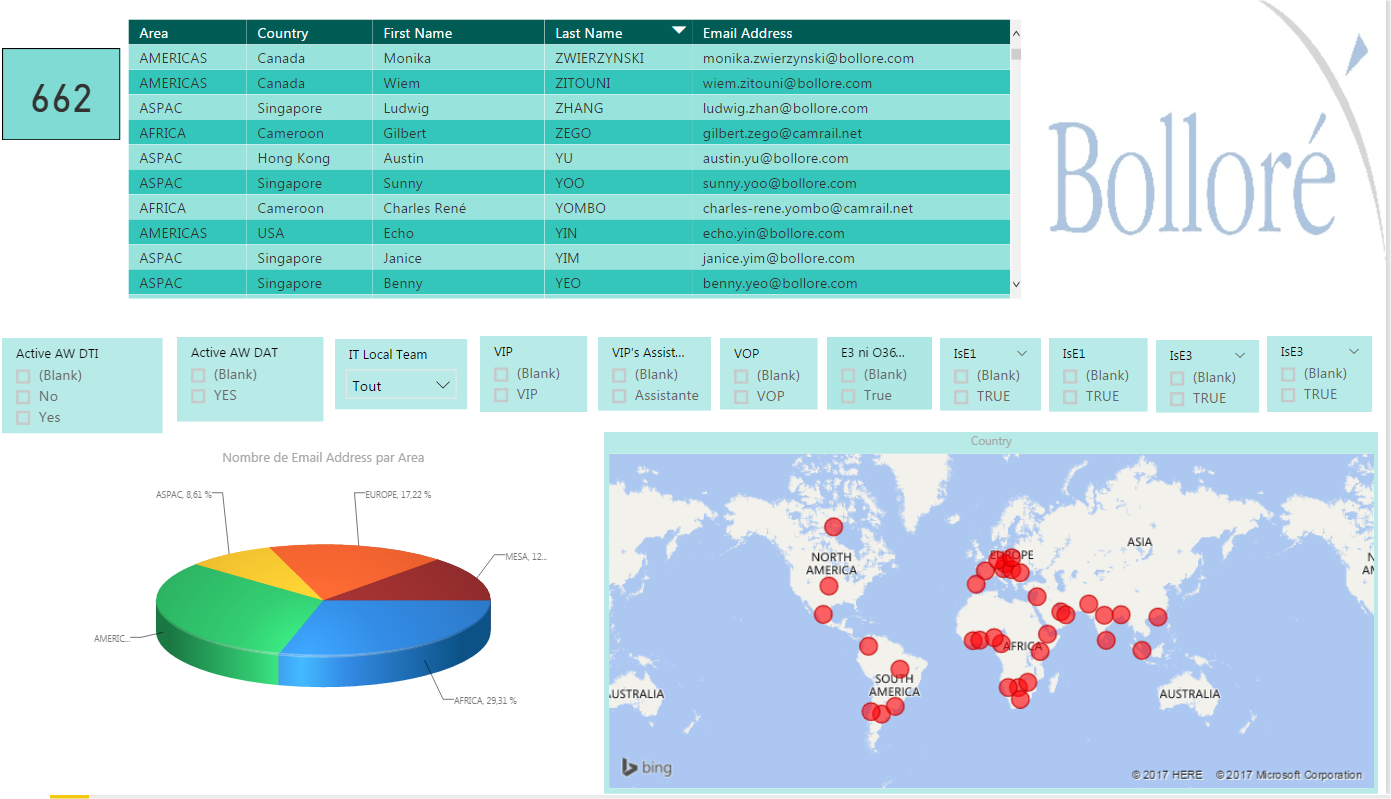
\includegraphics[width=1\linewidth]{Projet_O365/TB}
\end{center}
	\caption{Exemple sur un tableau de bord réalisé sous POWER BI sur 662 boites mail migrées}
	\label{fig:19}	
\end{figure}

\begin{figure}[H]
	\begin{center}
		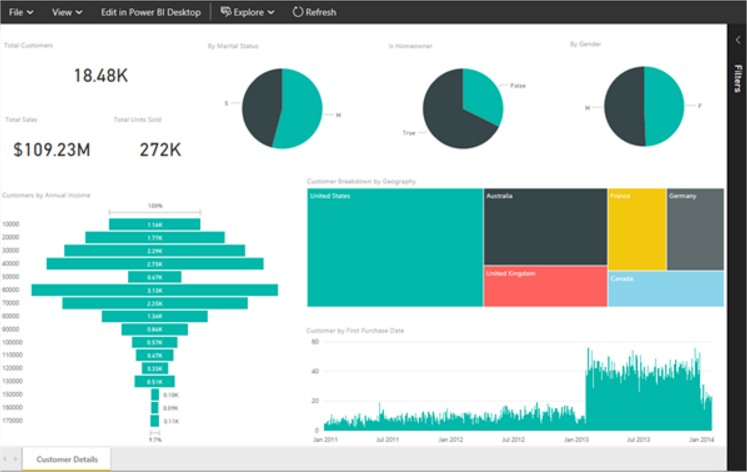
\includegraphics[width=1\linewidth]{Projet_O365/rapport_bi}
\end{center}
	\caption{Exemple sur un rapport réalisé sous POWER BI }
	\label{fig:20}	
\end{figure}

\begin{figure}[H]
	\begin{center}
		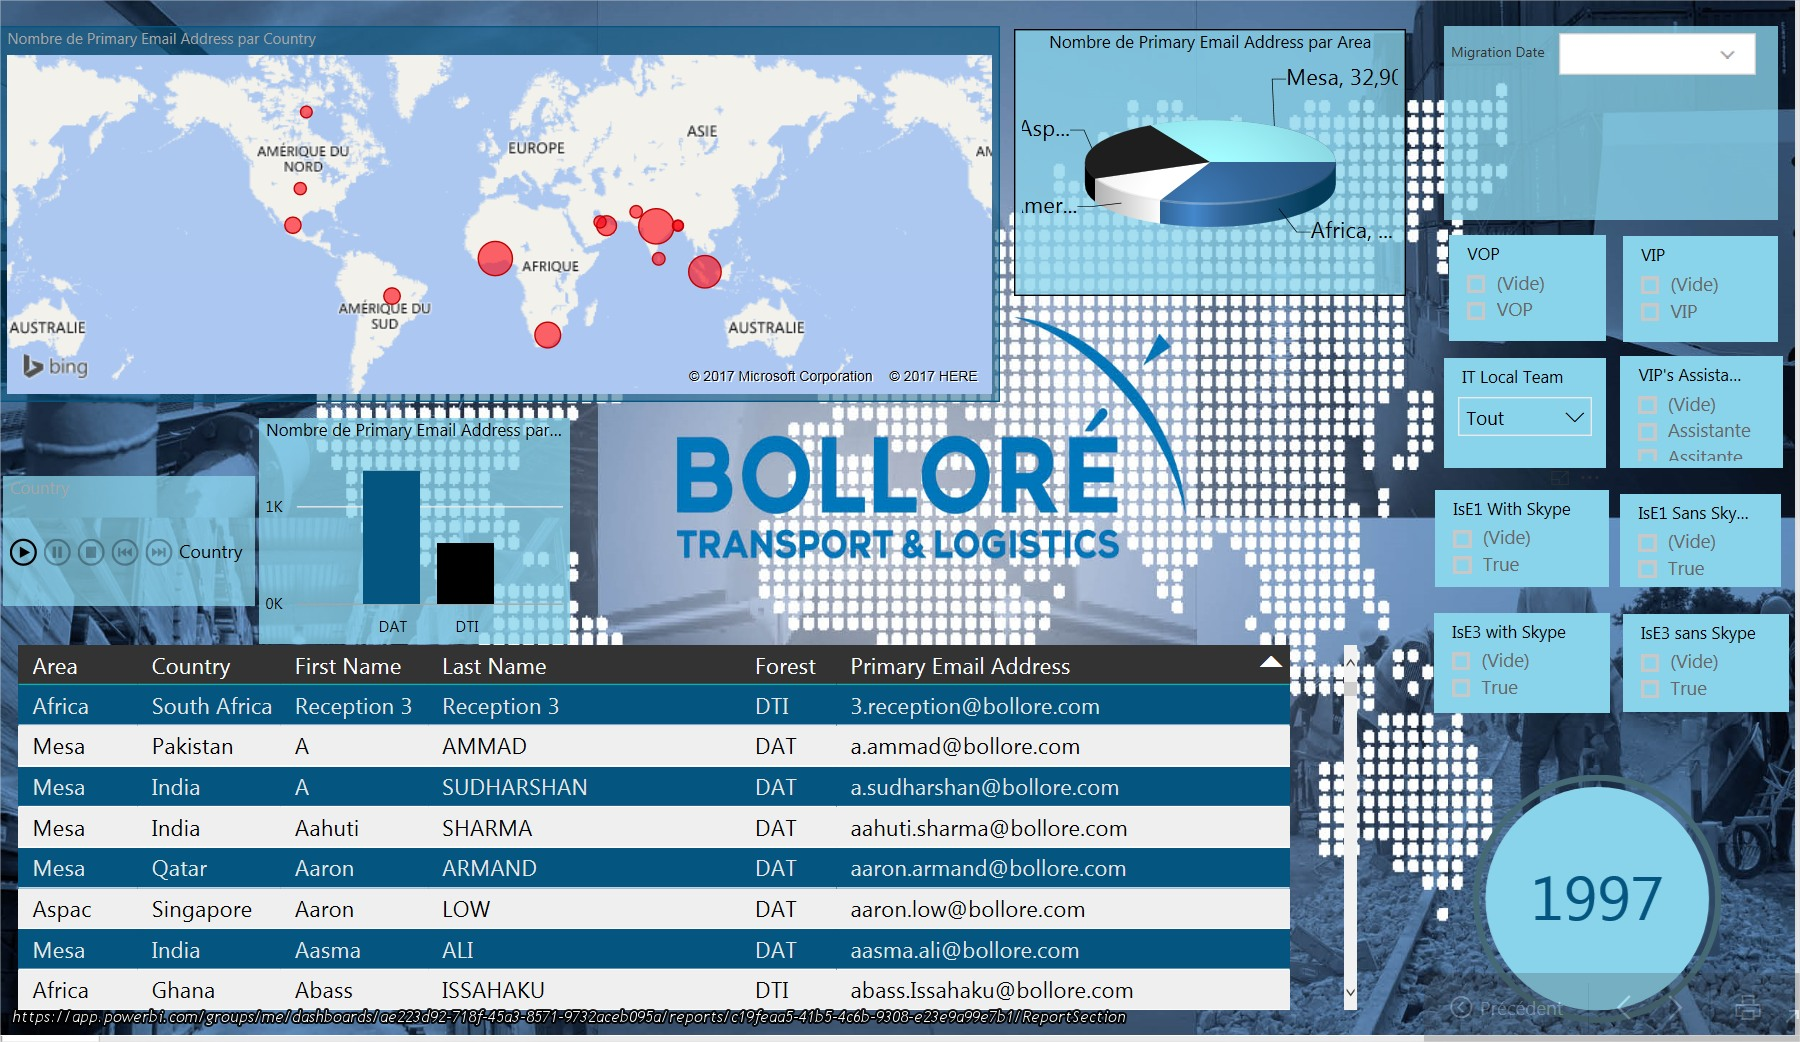
\includegraphics[width=1\linewidth]{Projet_O365/TB1}
\end{center}
	\caption{Exemple sur un tableau de bord réalisé sur 1997 adresses migrées }
	\label{fig:21}	
\end{figure}


\subsection*{Publication \& Partage }
\textcolor{black}{Une fois les outils de restitution sont créés et publiés sur l’espace de travail personnel, nous pouvons les partager avec d’autres collaborateurs qui auront la possibilité de les consulter et d’exporter les données concernées.}
~~\\

\textcolor{black}{Voici 2 captures sur un exemple de publication et de partage depuis l'espace de travail personnel.}
\begin{figure}[H]
	\begin{center}
		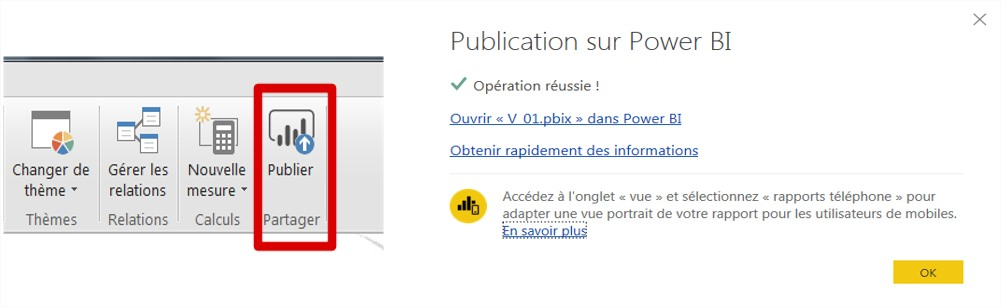
\includegraphics[width=1\linewidth]{Projet_O365/pub}
\end{center}
	\caption{ Exemple sur une publication d'un tableau de bord }
	\label{fig:21}	
\end{figure}

\begin{figure}[H]
	\begin{center}
		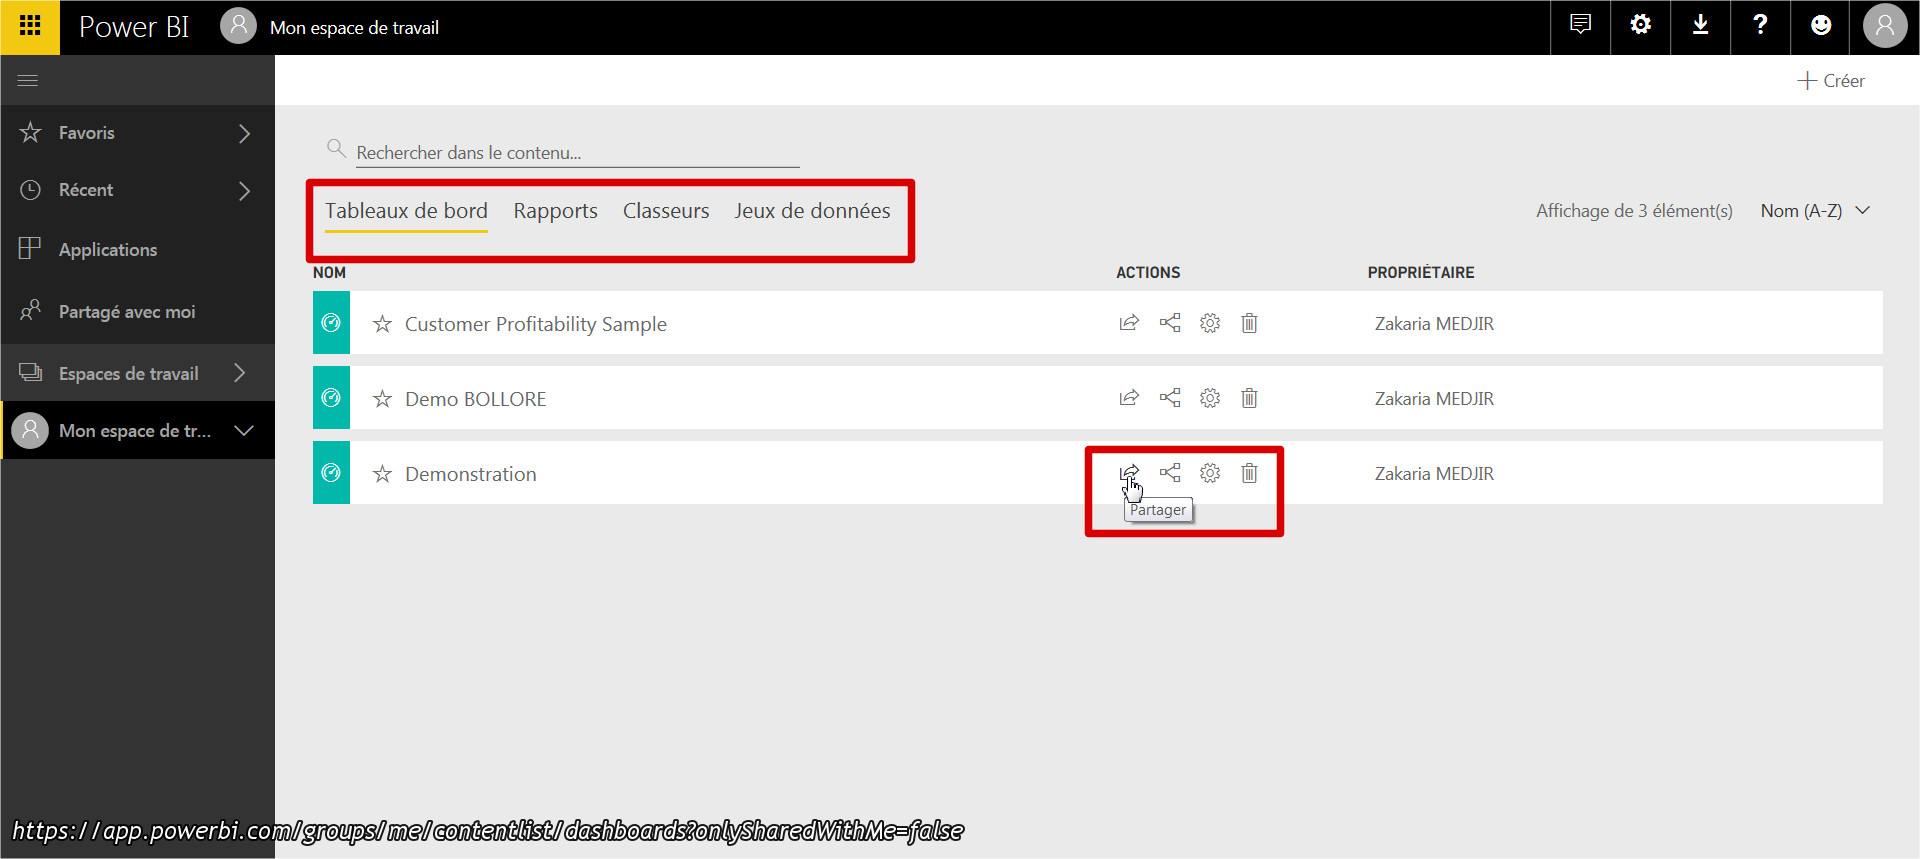
\includegraphics[width=1\linewidth]{Projet_O365/share}
\end{center}
	\caption{ Exemple sur la possibilité de partager un tableau de bord}
	\label{fig:22}	
\end{figure}
~~\\
\section{Compétences déployées}



\textcolor{Plusieurs compétences ont été déployées afin de bien effectuer les taches données et réussir les missions et les activité décrites précédemment. Ces compétences peuvent être regroupées en quatre catégorie :}

\begin{itemize}
	\item \textbf{Compétences techniques :} ~~\\
     \textcolor{black}{Les bases techniques dans la gestion des logiciels d’administration et de supervision et dans la gestion de projet ainsi que la maitrise des outils décisionnels (outils BI) ont rendu le travail moins difficile.}

    \item \textbf{Compétences fonctionnelles :} ~~\\
     \textcolor{black}{Les capacités de coordination, d’identification, d’analyse des données, de regroupement et d’interprétation des exigences sont les premiers facteurs clés de succès de certaines missions.}
     
     \item \textbf{Compétences organisationnelles :} ~~\\
     \textcolor{black}{L'organisation et la rigueur sont des qualités qui m’ont aidé à réussir ces missions. J’ai pu gérer mon temps en toute autonomie et respecter les délais qui ont été imposés. Aussi, anticiper l’organisation des ateliers de travail avec les différentes équipes m’a permis de consolider rapidement les besoins.}
     
     \item \textbf{Compétences relationnelles :} ~~\\
     \textcolor{black}{L’écoute et la disponibilité représentent également un secret de réussite. En effet, tout au long de ces missions j’ai été en contact direct avec des personnes différentes : les clients, les membres de l’équipe réseaux et télécommunication,des personnes travaillant dans differentes cellules internes et externes.}
\end{itemize}
~~\\

\section{Compétences requises}

\textcolor{Durant ce stage, j’ai eu l’occasion d’appliquer des connaissances déjà acquises et d’en développer de nouvelles ; de prouver que je pouvais être capable de m’adapter, d’exécuter, et de bien réaliser les taches de mon travail.
En effet, j’ai acquis de nombreuses compétences :}


\begin{itemize}
	\item \textbf{Sur le plan personnel :} 
	     \begin{itemize}
	      \item Elargir mes capacités d’adaptation et d’intégration. 
	      \item Pousser mon ouverture d’esprit et ma curiosité.
	      \item Consolider mon sens de responsabilité et mon autonomie.
	     \end{itemize}
	     
    \item \textbf{Sur le plan professionnel :} 
	     \begin{itemize}
	      \item Acquérir une véritable expérience professionnelle au travers d’un stage au sein d’une grande entreprise. 
	      \item Élargir mes compétences linguistes et mes façons de communication.
	      \item Appliquer les concepts théoriques déjà enseignés et maitriser les outils décisionnels.
	      \item Bien me préparer pour la carrière professionnelle.
	      \item Avoir une culture générale en informatique.
	      \item Être créatif pour trouver de nouvelles solutions.
	     \end{itemize}
\end{itemize}
